\chapter{Introduction}
\label{chap:intro} 
Throughout the history of software engineering, much effort has
been put on the description and understanding of high-level software 
processes. The waterfall model, the very 
first software process, has contributed to the success of many 
large software systems. High-level software processes divide the  
software development process into phases, where each phase lasts from a 
few days to several months \cite{Pfleeger:01,Pressman:03}. For example, the 
requirements analysis phase may last months before the design phase starts. 
Recently, increasing effort has been put on low-level software processes \cite{Larman:03,AgileAlliance}, in which a phase may last several minutes to 
a few hours only. Each phase defines how developers and development team 
should carry on the work on daily basis. The Personal Software Process 
(PSP) \cite{Humphrey:99} and Extreme Programming 
(XP) \cite{Jeffries:00,Beck:00,XP96} are two examples of a low-level 
software process. Although proven to be useful in improving software quality\cite{Ferguson:97,Kamatar:00,MicrosoftTSP,Janzen:05}, low-level 
software process are hard to execute correctly and repeatedly. In 
order to improve the quality of practice and research of low-level 
software process, there must be some supporting tools. In my 
dissertation research, I focus on one low-level software process, 
the called Test-Driven Development (TDD) \cite{Beck:03}, and I developed Zorro 
software system to study it.

Test-Driven Development (TDD) is an innovative one of the practices of Extreme
Programming. In TDD, the software development process is iterative and
incremental \cite{Larman:03}. There is only one task to accomplish in an
iteration. In a particular iteration, a unit test of the task is created
first followed by production code implementation.  TDD is built on the
foundation of the XUnit framework \cite{XUnit}, which has been ported to
more than 30 languages. Unit testing has become a de facto standard in the
software industry. TDD is widely adopted by software professionals. An
informal survey \cite{UnitTestingPoll:06} conducted by Method and Survey
magazine found that 46\% of the studied software organizations perform unit
testing informally, 41\% of the studied organizations document their unit
test cases, and 14\% of the studied organizations use the TDD approach.

``Clean code that works''\cite{Beck:03} is the goal of Test-Driven
Development. To achieve this goal, TDD summarizes its software development
process as two basic rules: ``(1) Write new code only if an automated test
has failed; (2) Eliminate duplication.''  Kent Beck, the pioneer of
Test-Driven Development, stated that there is an implicit order to software
development using TDD \cite{Beck:03}: 
\begin{enumerate}
\item Red - Write a little test that doesn't work, and perhaps doesn't even
  compile at first.
\item Green - Make the test work quickly, committing whatever sins are
  necessary in the process.  
\item Refactor - Eliminate all the duplication created by merely getting
  the test to work.  
\end{enumerate}
At first glimpse, TDD seems easy, but in fact, it is a very hard and
difficult low-level software process that requires much discipline to 
carry out correctly. First, software developers are not typically educated 
to write unit tests for the program they develop. Therefore,
in a lot of cases, software systems are not designed for easy testing.
Consequently, developers often find it is hard for them to write testing
code at all, much less write testing code prior to implementation. Second,
following the red/green/refactor software development pattern requires a
lot of effort. In TDD, software developers must continuously remain in the
mindset of test-first, which is initially counter-intuitive to many of them
\cite{Beck:01,Wang:04}. So they often apply it differently according to
their own experience level and understanding \cite{Beck:01}.

TDD is gradually becoming a standard well accepted for software development in industry,
and yet there are problems in testability and differences in understanding
of this methodology. Not surprisingly, the immaturity of TDD causes problems. 
There are many important research questions regarding software development using 
TDD. For example, how do we know software developers will faithfully commit
to the highly disciplined TDD practice? Will developers slip away from TDD?
When does it pay off to use TDD, and when does it not pay off? One thing is
clear: these questions cannot be answered accurately without good software
process measurement. However, Janzen and Saiedian \cite{Janzen:05} stated
that measuring the use of a software development methodology is hard. They
claimed it is so hard to do accurately that published data on the level of
TDD adoption in industry is either indirect or inaccurate \cite{Janzen:05,
  UnitTestingPoll:06}.  Fortunately, as my initial case study demonstrates,
measuring the use of certain software development methods is becoming
feasible with the emergence of technologies such as the Hackystat system
\cite{Hackystat:06,csdl2-04-11,csdl2-04-22,csdl2-03-12}, an in-process
software metrics collection and analysis framework.

As part of my dissertation research, I developed a software system
called Zorro (Figure \ref{fig:infra}) on top of Hackystat to infer TDD
development behaviors using low-level software development activity
data collected by Hackystat Eclipse Sensor.  Zorro recognizes and
evaluates TDD patterns using rule-based system support and the
software development stream analysis (SDSA) framework. SDSA is a
three-stage analysis technique that brings
the Hackystat framework and Zorro system together. First, it merges
software development activities and in-process metric data together to
create a ``software development stream'', a sequential stream of
low-level software development activities. Second, SDSA includes a
tokenization subsystem that divides a single sequential stream of
low-level software development activities into collections of events
called ``software development episodes''. Third, the JESS
\cite{Friedman-Hill:03} rule-based system recognizes and classifies
these episodes according to the classification schema.  SDSA binds these
three components together to assist the measurement of software
development methods and low-level software process.
\begin{figure}[htbp]
  \centering
  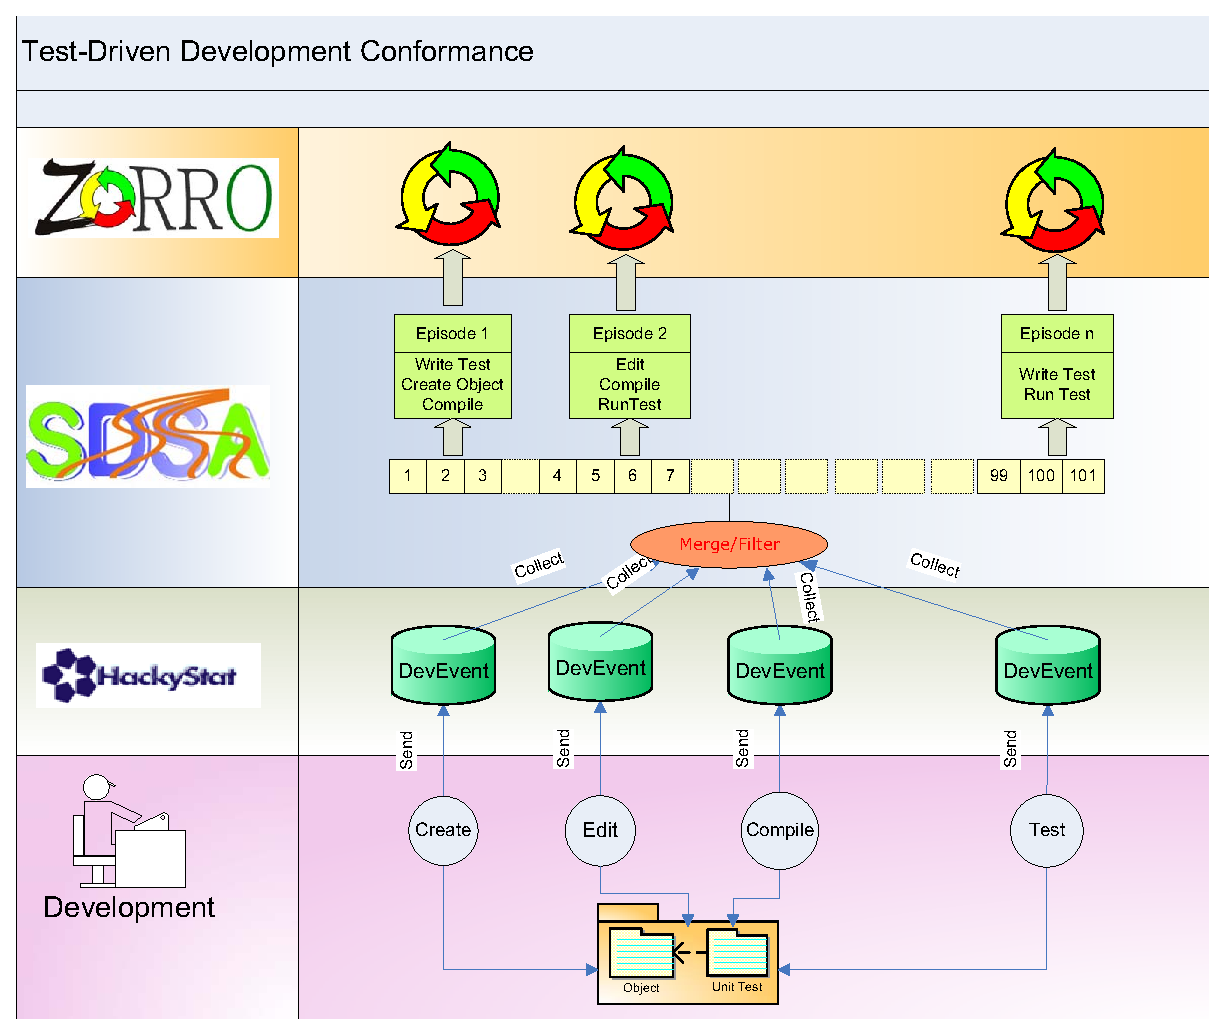
\includegraphics[width=0.9\textwidth]{figs/Zorro-Infrastructure.eps}
  \caption{Zorro Infrastructure}\label{fig:infra}
\end{figure}

With the capabilities provided by SDSA, I defined a set of specific rules
for TDD in Zorro according to Beck \cite{Beck:01,Beck:03} and others who have
described the practices of TDD. Zorro uses a two-step procedure to measure
and evaluate the compliance of the developer's behaviors with the practices
of TDD.  First, Zorro recognizes and classifies the episodes independently
according to the classification schema. Second, Zorro evaluates the
internal structure as well as the context of the episodes to deduce whether
an episode is TDD conformant or not.
















